%==============================================================================
%  Starting a PhD in ML / NLP -- slide deck
%  Konstantinos Skianis, University of Ioannina
%  Compile: latexmk -pdf phd-ml-nlp-slides.tex
%==============================================================================
\documentclass[aspectratio=169,11pt]{beamer}

\usepackage[T1]{fontenc}
\usepackage[utf8]{inputenc}
\usepackage{lmodern}
\usepackage{microtype}
\usepackage{xcolor}
\usepackage{booktabs,array,tabularx,colortbl}
\usepackage{tikz}
\usetikzlibrary{arrows.meta,positioning,shapes.geometric}
\usepackage{amsmath,amssymb}

%--------------------------------------------------------------- appearance ---
\usetheme{default}
\usefonttheme{professionalfonts}
\setbeamertemplate{navigation symbols}{}

\definecolor{brand}{HTML}{1F4E79}
\definecolor{brandlight}{HTML}{2E7BB8}
\definecolor{accent}{HTML}{B5451B}
\definecolor{ink}{HTML}{22262B}
\definecolor{mutegray}{HTML}{5A6472}
\definecolor{rowtint}{HTML}{EFF4F9}
\definecolor{boxtint}{HTML}{F3F7FB}

\setbeamercolor{structure}{fg=brand}
\setbeamercolor{normal text}{fg=ink}
\setbeamercolor{frametitle}{fg=brand}
\setbeamercolor{itemize item}{fg=brandlight}
\setbeamercolor{itemize subitem}{fg=brandlight}
\setbeamercolor{enumerate item}{fg=brandlight}
\setbeamerfont{frametitle}{size=\large,series=\bfseries}
\setbeamertemplate{itemize item}{\small\raise0.5pt\hbox{\textbullet}}
\setbeamertemplate{itemize subitem}{\footnotesize\raise0.5pt\hbox{--}}
\setbeamertemplate{section in toc}{\inserttocsectionnumber.~\inserttocsection}

% frame title with rule
\setbeamertemplate{frametitle}{%
  \vspace{6pt}%
  \begin{beamercolorbox}[wd=\paperwidth,leftskip=0.9cm,rightskip=0.9cm]{frametitle}%
    \usebeamerfont{frametitle}\insertframetitle%
    \ifx\insertframesubtitle\empty\else
      \\[1pt]{\small\normalfont\color{mutegray}\insertframesubtitle}%
    \fi
    \par\vspace{3pt}{\color{brandlight}\rule{\dimexpr\paperwidth-1.8cm\relax}{1pt}}%
  \end{beamercolorbox}%
}

% footline
\setbeamertemplate{footline}{%
  \hbox{\begin{beamercolorbox}[wd=\paperwidth,ht=2.6ex,dp=1.4ex,leftskip=0.9cm,rightskip=0.9cm]{}%
  \tiny\color{mutegray}Starting a PhD in ML / NLP \quad\textbullet\quad K. Skianis, Univ.\ of Ioannina
  \hfill\insertframenumber/\inserttotalframenumber
  \end{beamercolorbox}}%
}

\setbeamercolor{block title}{bg=boxtint,fg=brand}
\setbeamercolor{block body}{bg=boxtint,fg=ink}
\setbeamercolor{block title alerted}{bg=accent!10,fg=accent}
\setbeamercolor{block body alerted}{bg=accent!10,fg=ink}
\setbeamertemplate{blocks}[rounded][shadow=false]

\newcommand{\code}[1]{\texttt{\small #1}}
\newcommand{\lnk}[2]{\href{#1}{\color{brandlight}\underline{#2}}}
\newcommand{\key}[1]{\textbf{\color{brand}#1}}
\renewcommand{\arraystretch}{1.15}

% section divider slides
\AtBeginSection[]{%
  \begin{frame}[plain,noframenumbering]
    \vfill
    \begin{center}
      {\color{brandlight}\rule{0.72\textwidth}{1.4pt}}\\[10pt]
      {\small\color{mutegray}Part \insertsectionnumber}\\[4pt]
      {\LARGE\bfseries\color{brand}\insertsectionhead}\\[10pt]
      {\color{brandlight}\rule{0.72\textwidth}{1.4pt}}
    \end{center}
    \vfill
  \end{frame}}

%------------------------------------------------------------------ titles ----
\title{\bfseries Starting a PhD in Machine Learning or NLP}
\subtitle{Venues, deadlines, tools, and the habits that compound}
\author{Konstantinos Skianis}
\institute{Assistant Professor of Natural Language Processing\\
Department of Computer Science and Engineering, University of Ioannina\\[2pt]
\small\lnk{https://y3nk0.github.io}{y3nk0.github.io}}
\date{October 2026}

\begin{document}

%==============================================================================
\begin{frame}[plain,noframenumbering]
  \vspace{0.3cm}
  {\color{brandlight}\rule{\textwidth}{2pt}}\\[14pt]
  {\LARGE\bfseries\color{brand}Starting a PhD in\\[4pt] Machine Learning or NLP}\\[8pt]
  {\large\color{ink}Venues, deadlines, tools, and the habits that compound}\\[10pt]
  {\color{brandlight}\rule{\textwidth}{2pt}}\\[14pt]
  {\bfseries Konstantinos Skianis}\\[3pt]
  {\small\color{mutegray}Assistant Professor of Natural Language Processing\\
  Department of Computer Science and Engineering, University of Ioannina}\\[4pt]
  {\small\lnk{https://y3nk0.github.io}{y3nk0.github.io}}
  \vfill
  {\footnotesize\color{mutegray}October 2026 \quad\textbullet\quad companion to the
  full starter guide and the one-page cheat sheet}
\end{frame}

%==============================================================================
\begin{frame}{What this deck is}
\begin{columns}[T]
\begin{column}{0.56\textwidth}
A PhD is won on \key{compounding habits}, not heroic sprints.


\medskip
The first 90 days decide how much friction every later month carries:
\begin{itemize}
  \item Can you find, in November, the paper you read in March?
  \item Can you rerun the experiment behind Table 3?
  \item Can anyone find \emph{you}?
  \item Does a deadline ever surprise you?
\end{itemize}
\end{column}
\begin{column}{0.42\textwidth}
\begin{block}{Roadmap}
\footnotesize
\begin{enumerate}
  \item Venues: where your work goes
  \item Deadlines
  \item Writing \& sharing
  \item Zotero
  \item Your first project: a survey
  \item Searching the literature
  \item Reading the signals
  \item AI assistant
  \item Your personal site
  \item Infrastructure \& habits
\end{enumerate}
\end{block}
\end{column}
\end{columns}
\end{frame}

%==============================================================================
\begin{frame}{The first 90 days, condensed}
\begin{columns}[T]
\begin{column}{0.33\textwidth}
\begin{block}{Week 1 --- infrastructure}
\scriptsize
Zotero + Better BibTeX\\
Scholar profile + 3 alerts\\
Accounts: Overleaf, Prism, OpenReview, GitHub, HF, arXiv, ORCID\\
Deadlines in the calendar\\
AI assistant + memory file\\
One repo per project, with \code{notes/}
\end{block}
\end{column}
\begin{column}{0.33\textwidth}
\begin{block}{Weeks 2--10 --- a survey}
\scriptsize
A narrow question, agreed in writing.\\[4pt]
Output: 60--120 papers screened, an extraction sheet, a taxonomy figure,
10--15 pages written, \key{three gaps} stated as testable questions.\\[4pt]
The highest-return thing you can do in term one.
\end{block}
\end{column}
\begin{column}{0.33\textwidth}
\begin{block}{Weeks 10--13 --- identity}
\scriptsize
Publish \code{username.github.io}\\[4pt]
Reproduce \emph{one} baseline end to end, tracked, on your own hardware\\[4pt]
Pick a target venue and backward-plan from its deadline
\end{block}
\end{column}
\end{columns}
\end{frame}

%==============================================================================
\section{The publication landscape}

\begin{frame}{ML and NLP are conference-first}
\begin{columns}[T]
\begin{column}{0.55\textwidth}
\begin{enumerate}
  \item \key{Cycles, not rolling submissions.} One or two hard deadlines per
        year. Miss by an hour, wait months.
  \item \key{Reviewing is public-ish.} ICLR and many workshops review on
        OpenReview --- reviews and rebuttals stay online.
  \item \key{A paper has a lifecycle.} 6--12 months from idea to published.
\end{enumerate}
\end{column}
\begin{column}{0.44\textwidth}
\begin{block}{The lifecycle}
\footnotesize
preprint $\rightarrow$ submission $\rightarrow$ reviews $\rightarrow$
\textbf{rebuttal} $\rightarrow$ decision $\rightarrow$ camera-ready
$\rightarrow$ talk / poster $\rightarrow$ citations
\end{block}
\begin{alertblock}{Read other people's reviews}
\footnotesize
OpenReview is the best free writing lesson in the field. Read the reviews and
rebuttals of papers near your topic \emph{before} you write yours.
\end{alertblock}
\end{column}
\end{columns}
\end{frame}

%------------------------------------------------------------------------------
\begin{frame}{Core ML venues}{Dates are indicative patterns --- verify every year}
\footnotesize
\begin{tabularx}{\textwidth}{>{\raggedright\arraybackslash}p{2.1cm} X >{\raggedright\arraybackslash}p{3.5cm}}
\toprule
\textbf{\color{brand}Venue} & \textbf{\color{brand}Scope} & \textbf{\color{brand}Rhythm} \\
\midrule
\rowcolor{rowtint}
NeurIPS & Broadest ML: theory, deep learning, datasets \& benchmarks & abstract $\sim$May; December \\
ICML & Core ML, methods and theory & $\sim$Jan--Feb; July \\
\rowcolor{rowtint}
ICLR & Representation learning, LLMs; fully open review & $\sim$Sept; April--May \\
AISTATS & Statistics $\times$ ML & $\sim$Oct; April--May \\
\rowcolor{rowtint}
COLT / UAI & Learning theory / probabilistic \& causal & winter--spring \\
AAAI / IJCAI & Broad AI and applications & $\sim$Aug / $\sim$Jan \\
\rowcolor{rowtint}
COLM & Language modelling: data, training, evaluation & $\sim$March; October \\
MLSys / LoG & Systems for ML / learning on graphs & autumn \\
\bottomrule
\end{tabularx}
\end{frame}

%------------------------------------------------------------------------------
\begin{frame}{Core NLP venues}
\footnotesize
\begin{tabularx}{\textwidth}{>{\raggedright\arraybackslash}p{2.4cm} X >{\raggedright\arraybackslash}p{3.2cm}}
\toprule
\textbf{\color{brand}Venue} & \textbf{\color{brand}Scope} & \textbf{\color{brand}Notes} \\
\midrule
\rowcolor{rowtint}
ACL & The flagship: all of CL and NLP & summer; via ARR \\
EMNLP & Empirical methods --- the other flagship & late year; via ARR \\
\rowcolor{rowtint}
NAACL / EACL / AACL & Regional ACL conferences, same standard & alternate by year \\
COLING / LREC & CL / language resources and evaluation & check the current cycle \\
\rowcolor{rowtint}
CoNLL / *SEM / SemEval & Learning and language, semantics, shared tasks & good first-paper targets \\
Interspeech / ICASSP & Speech and audio & own cycles \\
\rowcolor{rowtint}
TACL & Journal of the ACL, rolling; presented at *ACL & slower, prestigious \\
Findings & Companion archival track for solid papers & a real, citable publication \\
\bottomrule
\end{tabularx}
\end{frame}

%------------------------------------------------------------------------------
\begin{frame}{ARR: the mechanic that confuses every first-year}
\centering
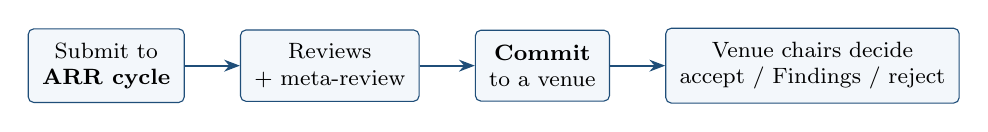
\begin{tikzpicture}[node distance=7mm,
  box/.style={draw=brand,fill=boxtint,rounded corners=2pt,inner sep=5pt,
              align=center,font=\footnotesize,minimum height=9mm},
  arr/.style={-{Stealth[length=2mm]},brand,thick}]
\node[box] (sub) {Submit to\\\textbf{ARR cycle}};
\node[box,right=of sub] (rev) {Reviews\\+ meta-review};
\node[box,right=of rev] (com) {\textbf{Commit}\\to a venue};
\node[box,right=of com] (dec) {Venue chairs decide\\accept / Findings / reject};
\draw[arr] (sub)--(rev); \draw[arr] (rev)--(com); \draw[arr] (com)--(dec);
\end{tikzpicture}

\vspace{4mm}
\begin{columns}[T]
\begin{column}{0.48\textwidth}
\begin{block}{Plan around this}
\footnotesize
\textbf{Two} deadlines: ARR submission \emph{and} venue commitment.\\[3pt]
Reviews are reusable: revise and commit elsewhere, or resubmit with a revision
note.
\end{block}
\end{column}
\begin{column}{0.48\textwidth}
\begin{alertblock}{Desk-reject risks}
\footnotesize
A \key{Limitations} section is mandatory (and free of page limit).\\[3pt]
So is the Responsible NLP checklist.
\end{alertblock}
\end{column}
\end{columns}
\end{frame}

%------------------------------------------------------------------------------
\begin{frame}{Where a first paper realistically lands}
\begin{columns}[T]
\begin{column}{0.52\textwidth}
\textbf{Adjacent venues}\\
\footnotesize KDD, WSDM, CIKM, SIGIR, The Web Conference, ECML-PKDD $\cdot$
CVPR / ICCV / ECCV for multimodal work.
\medskip

\normalsize\textbf{Journals}\\
\footnotesize JMLR $\cdot$ \key{TMLR} --- rolling, fast, judged on correctness
and interest rather than novelty hype; an excellent fit for careful work
conference reviewers undervalue $\cdot$ TACL $\cdot$ \emph{Computational
Linguistics} $\cdot$ TPAMI.
\end{column}
\begin{column}{0.46\textwidth}
\begin{block}{Aim your first submission at a good workshop}
\footnotesize
4--8 pages, fast turnaround, real feedback, real audiences.\\[4pt]
You learn the entire pipeline --- writing, reviewing, rebuttal, poster,
conversations --- at a fraction of the risk.
\end{block}
\end{column}
\end{columns}
\end{frame}

%------------------------------------------------------------------------------
\begin{frame}{Judging a venue without asking around}
\begin{columns}[T]
\begin{column}{0.56\textwidth}
\begin{itemize}
  \item \key{Google Scholar Metrics} --- per-venue h5-index.
  \item \key{CORE ranking} --- A*/A/B/C tiers, used for evaluation in many
        countries.
  \item \key{CSRankings} --- which venues count as top-tier \emph{per subarea}:
        the useful signal.
  \item \key{Where does the work you admire appear?} The most reliable test.
\end{itemize}
\end{column}
\begin{column}{0.42\textwidth}
\begin{alertblock}{Predatory venues}
\footnotesize
Invitation email $+$ acceptance in two weeks $+$ a large fee $+$ a scope
spanning ``AI, Big Data, Blockchain and IoT'' $=$ a scam.\\[4pt]
Publishing there actively damages your CV.
\end{alertblock}
\end{column}
\end{columns}
\end{frame}

%==============================================================================
\section{Deadlines}

\begin{frame}{Two boards to bookmark}
\begin{block}{1. Papers with Code --- AI Deadlines \quad \lnk{https://paperswithcode.co/ai-deadlines}{paperswithcode.co/ai-deadlines}}
\footnotesize
Run by Hugging Face. Filter by subfield (ML, NLP, CV, DM, Robotics, IR,
Speech, RL, \ldots) or \emph{top tier only}. Tracks \key{every} milestone ---
abstract registration, reviews released, author feedback, rebuttal,
commitment, notification, camera-ready --- with live countdowns, conference
dates and locations. API + MCP endpoint for your assistant.
\end{block}
\begin{block}{2. AI Deadlines, pre-filtered \quad \lnk{http://aideadlines.org/?sub=ML,CV,NLP}{aideadlines.org/?sub=ML,CV,NLP}}
\footnotesize
The \code{sub=} parameter carries the filter, so the link \emph{is} your
personalised board --- edit the tags as your interests change. Mirrored as a
Hugging Face Space; the data is open YAML, so a missing deadline is a pull
request away: an easy first open-source contribution.
\end{block}
\centering\footnotesize
\key{AoE $=$ UTC$-$12.} Cross-check both against the official venue page ---
aggregators lag, calls for papers do not.
\end{frame}

%------------------------------------------------------------------------------
\begin{frame}{A workflow that actually holds}
\begin{columns}[T]
\begin{column}{0.5\textwidth}
\begin{enumerate}
  \item Filter to your subfields; list the 4--6 venues you could target in 18
        months.
  \item Calendar each one \key{three times}: the deadline, $-7$ days (results
        frozen, writing only), $-21$ days (experiments running).
  \item Add the dates people forget: abstracts, ARR commitment,
        supplementary, \key{rebuttal window} (do not travel), camera-ready,
        early registration.
\end{enumerate}
\end{column}
\begin{column}{0.48\textwidth}
\begin{block}{Backward-plan on paper}
\footnotesize
camera-ready $\leftarrow$ decision $\leftarrow$ rebuttal $\leftarrow$
submission $\leftarrow$ freeze $\leftarrow$ final experiments $\leftarrow$
\textbf{ablations} $\leftarrow$ main result\\[4pt]
Ablations always take longer than the main result.
\end{block}
\begin{alertblock}{In moderation}
\footnotesize
Deadlines are useful forcing functions and terrible research strategies. Keep
one long-horizon question alive alongside them --- that is where your thesis
contribution comes from.
\end{alertblock}
\end{column}
\end{columns}
\end{frame}

%==============================================================================
\section{Writing and sharing}

\begin{frame}{Where you write}
\begin{columns}[T]
\begin{column}{0.48\textwidth}
\begin{block}{Overleaf \quad\footnotesize\lnk{https://www.overleaf.com}{overleaf.com}}
\footnotesize
\begin{itemize}
  \item Real-time co-editing --- what you want in the 48 hours before a
        deadline.
  \item Official venue templates in the gallery: \emph{start from them}, not
        from last year's copy.
  \item Comments and chat for advisor feedback.
  \item Check for an institutional licence before paying; the free tier limits
        collaborators, compile time, history, Git sync.
\end{itemize}
\end{block}
\end{column}
\begin{column}{0.48\textwidth}
\begin{block}{Prism \quad\footnotesize\lnk{https://prism.openai.com}{prism.openai.com}}
\footnotesize
\begin{itemize}
  \item OpenAI's AI-native LaTeX workspace (January 2026).
  \item Free: unlimited projects, collaborators, compile time.
  \item The model sees the \emph{whole} manuscript --- sections, equations,
        citations, the argument.
  \item Strong at prose, tables, LaTeX errors you cannot find, and levelling
        the field for non-native English writers.
\end{itemize}
\end{block}
\end{column}
\end{columns}
\end{frame}

%------------------------------------------------------------------------------
\begin{frame}{Two cautions, and the local workflow}
\begin{columns}[T]
\begin{column}{0.48\textwidth}
\begin{alertblock}{Before moving your thesis into any AI editor}
\footnotesize
\key{Policy:} most venues have an explicit AI-assistance policy --- disclosure
requirements, and a hard ban on LLM-written \emph{reviews}. You remain
responsible for every sentence, citation and number.\\[4pt]
\key{Confidentiality:} never upload NDA'd data, industry collaborations, or
someone else's unpublished work.
\end{alertblock}
\end{column}
\begin{column}{0.48\textwidth}
\begin{block}{Keep a local copy too}
\footnotesize
\begin{itemize}
  \item \code{git} + \code{latexmk -pdf -pvc} + VS Code.
  \item \key{One sentence per line} --- turns git diffs from useless to
        invaluable.
  \item \code{\textbackslash input} per section, so two people do not collide.
  \item Figures generated by a script from logged results. Never hand-edited.
\end{itemize}
\end{block}
\end{column}
\end{columns}
\end{frame}

%------------------------------------------------------------------------------
\begin{frame}{Preprints, anonymity, artefacts}
\begin{columns}[T]
\begin{column}{0.5\textwidth}
\begin{itemize}
  \item \key{arXiv} --- cs.CL, cs.LG, cs.AI, stat.ML. First submission needs
        endorsement; your advisor handles it.
  \item \key{Anonymity:} ACL venues enforce a window around the review cycle;
        ML venues are double-blind but usually allow preprints. \emph{Check
        before you post.}
  \item Anonymise code too
        (\lnk{https://anonymous.4open.science}{anonymous.4open.science}), and
        strip names from PDF metadata.
\end{itemize}
\end{column}
\begin{column}{0.48\textwidth}
\begin{block}{Run this every time}
\footnotesize
\lnk{https://github.com/google-research/arxiv-latex-cleaner}{arxiv-latex-cleaner}
strips comments, unused files and bloat.\\[3pt]
Reviewers have found deanonymising information in LaTeX comments.
\end{block}
\begin{block}{Artefacts}
\footnotesize
Code on GitHub with a licence, checkpoints and data on Hugging Face, an exact
environment spec --- and an \key{ORCID} on everything.
\end{block}
\end{column}
\end{columns}
\end{frame}

%==============================================================================
\section{Zotero}

\begin{frame}{Set this up before paper number ten}
\begin{columns}[T]
\begin{column}{0.52\textwidth}
\textbf{The setup, in order}
\begin{enumerate}\footnotesize
  \item \key{Zotero} desktop + the browser \key{connector} --- one click saves
        metadata \emph{and} the PDF.
  \item \key{Better BibTeX}: pinned citation keys
        (\code{devlin2019bert}) and \key{auto-export} into your repo's
        \code{paper/refs.bib}. Never hand-edit BibTeX again.
  \item Sync (300\,MB free, or your own WebDAV / linked folder).
  \item A \key{group library} with your lab and co-authors.
  \item Collections per project, tags per theme, saved searches.
  \item Read and annotate \emph{inside} Zotero --- highlights stay searchable
        for years.
\end{enumerate}
\end{column}
\begin{column}{0.46\textwidth}
\begin{block}{Habits that keep it trustworthy}
\footnotesize
\begin{itemize}
  \item \key{Cite the published version}, not the preprint.
  \item Clean BibTeX from \key{DBLP} and the \key{ACL Anthology} --- Scholar's
        is sloppy about venues, pages, editors.
  \item Add items by DOI / arXiv ID.
  \item Merge duplicates monthly.
  \item One-sentence note on save: what it does, why I care.
\end{itemize}
\end{block}
\footnotesize
Overleaf's paid tiers link Zotero directly --- but auto-export into git is
better anyway: versioned, diffable, identical for every co-author.
\end{column}
\end{columns}
\end{frame}

%------------------------------------------------------------------------------
\begin{frame}{Getting a reference into your \code{.bib}}
\begin{columns}[T]
\begin{column}{0.5\textwidth}
\begin{block}{The easiest route --- no setup}
\footnotesize
\begin{enumerate}
  \item Google Scholar: \emph{Settings} $\rightarrow$ \emph{Bibliography
        manager} $\rightarrow$ tick \emph{Show links to import citations into
        BibTeX}. Once, ever.
  \item A \key{Cite} link appears under every result $\rightarrow$
        \key{BibTeX} $\rightarrow$ copy.
  \item Paste into \code{refs.bib}, or into Zotero with \emph{File
        $\rightarrow$ Import from clipboard}.
\end{enumerate}
Bulk: star papers into \emph{My library}, select, \emph{Export} $\rightarrow$
\emph{BibTeX}.
\end{block}
\end{column}
\begin{column}{0.48\textwidth}
\begin{alertblock}{Check what it gives you}
\footnotesize
``arXiv preprint arXiv:1810.04805'' for a paper published at NAACL, missing
pages, inconsistent venue names, mangled accents. A bibliography full of
``arXiv preprint'' says nobody looked.
\end{alertblock}
\footnotesize
\textbf{Cleaner, one click each:} \key{ACL Anthology} (per paper, and a
\code{.bib} per volume) $\cdot$ \key{DBLP} $\cdot$ \key{arXiv} ``Export
BibTeX'' $\cdot$ Semantic Scholar, ACM, IEEE, Springer.\\[3pt]
\textbf{Any DOI, from the terminal:}\\
\code{curl -LH "Accept: application/x-bibtex"}\\
\code{https://doi.org/<DOI>}\\[3pt]
Past $\sim$20 refs: connector + Better BibTeX auto-export does it all.
\end{column}
\end{columns}
\end{frame}

%==============================================================================
\section{Your first project: a focused survey}

\begin{frame}{Why a survey is the right first project}
\begin{columns}[T]
\begin{column}{0.52\textwidth}
\begin{itemize}
  \item \key{Vocabulary} --- you can talk to your advisor as a peer within
        weeks.
  \item \key{A taxonomy} --- and your first paper usually lives in a box you
        drew that has nothing in it.
  \item \key{A bibliography} you reuse in every paper and in your thesis.
  \item \key{Baselines, datasets, metrics} --- learned before you waste a
        month on a non-standard setup.
  \item \key{Publishable}: a survey, a position paper, a workshop paper, and
        the core of your related-work chapter.
\end{itemize}
\end{column}
\begin{column}{0.46\textwidth}
\begin{block}{The deliverables}
\footnotesize
\begin{itemize}
  \item 60--120 papers screened and extracted
  \item An annotated bibliography in Zotero
  \item An extraction spreadsheet
  \item One taxonomy figure
  \item 10--15 pages of writing
  \item \key{Three gaps}, each a testable question plus the experiment that
        would answer it
\end{itemize}
\end{block}
\centering\footnotesize 8--12 weeks. Timeboxed.
\end{column}
\end{columns}
\end{frame}

%------------------------------------------------------------------------------
\begin{frame}{A protocol you can run}
\begin{columns}[T]
\begin{column}{0.49\textwidth}
\footnotesize
\begin{enumerate}
  \item \key{Write the question down.} Not ``LLM reasoning'' but ``methods for
        verifying intermediate reasoning steps, 2022--2026, and how they are
        evaluated''. Agree it in writing.
  \item \key{Seed set:} 5--10 anchor papers from your advisor. Their shared
        vocabulary becomes your queries.
  \item \key{Criteria} for inclusion and exclusion, written \emph{before}
        screening --- or you will rationalise.
  \item \key{Search systematically} across Scholar, Semantic Scholar, the
        Anthology, OpenReview, DBLP --- and \key{log every query, date and hit
        count}.
  \item \key{Snowball both ways:} backward through references, forward through
        ``cited by''. Forward finds the last six months.
\end{enumerate}
\end{column}
\begin{column}{0.49\textwidth}
\footnotesize
\begin{enumerate}\setcounter{enumi}{5}
  \item \key{Screen in two passes:} title + abstract (ruthless, keep a
        ``maybe'' pile), then full text. Expect 400--600 screened, 60--120
        kept.
  \item \key{Extract into a table}, not prose. One row per paper.
  \item \key{Build the taxonomy.} Cluster until the groups stop changing. If
        you cannot draw it, you do not understand the field yet.
  \item \key{Write as you go} --- each section ends with ``what is missing
        here''.
  \item \key{Finish with three gaps.} Take them to your advisor; that meeting
        is where your first paper starts.
\end{enumerate}
\end{column}
\end{columns}
\end{frame}

%------------------------------------------------------------------------------
\begin{frame}{The extraction schema}{A spreadsheet 100 rows deep beats 100 highlighted PDFs}
\footnotesize
\begin{columns}[T]
\begin{column}{0.49\textwidth}
\begin{tabularx}{\textwidth}{>{\raggedright\arraybackslash}p{2.0cm} X}
\toprule
\rowcolor{rowtint} Key & pinned BibTeX key \\
Venue / year & published venue, not ``arXiv'' \\
\rowcolor{rowtint} Problem & the task, one line, your words \\
Method family & your taxonomy label \\
\rowcolor{rowtint} Data & datasets and sizes \\
Metrics & comparable across papers? \\
\bottomrule
\end{tabularx}
\end{column}
\begin{column}{0.49\textwidth}
\begin{tabularx}{\textwidth}{>{\raggedright\arraybackslash}p{2.1cm} X}
\toprule
\rowcolor{rowtint} Headline result & the number they lead with + the baseline \\
Compute & GPUs, hours, model size --- can \emph{you} run it? \\
\rowcolor{rowtint} Code & link + does it reproduce? \\
Limitations & stated and unstated \\
\rowcolor{rowtint} Relevance & 1--5 and ``why I care'' \\
\bottomrule
\end{tabularx}
\end{column}
\end{columns}
\vspace{3mm}
\begin{columns}[T]
\begin{column}{0.49\textwidth}
\begin{block}{Read in three passes (Keshav)}
\footnotesize
5 min: skim and decide $\rightarrow$ 1 h: figures, tables, method $\rightarrow$
hours: re-derive. Pass 3 for $\sim$20 papers; pass 1 for hundreds.
\end{block}
\end{column}
\begin{column}{0.49\textwidth}
\begin{alertblock}{Scope discipline}
\footnotesize
Freeze the search date (``literature up to 15 November 2026'') and ship. A
documented cut-off is exactly what a reviewer wants to see.
\end{alertblock}
\end{column}
\end{columns}
\end{frame}

%==============================================================================
\section{Searching the literature}

\begin{frame}{Google Scholar is an instrument, not a search box}
\footnotesize
\begin{tabularx}{\textwidth}{>{\raggedright\arraybackslash}p{4.6cm} X}
\toprule
\textbf{\color{brand}Query / feature} & \textbf{\color{brand}What it does} \\
\midrule
\rowcolor{rowtint} \code{"contrastive decoding"} & exact phrase --- always quote technical terms \\
\code{retrieval OR retrieve} & \code{OR} must be capitalised; fields rename themselves \\
\rowcolor{rowtint} \code{-survey -review} & exclude terms once surveys swamp results \\
\code{author:"K Skianis"} & author search; try initial + surname variants \\
\rowcolor{rowtint} \code{source:"Empirical Methods"} & search within a venue \\
\code{intitle:hallucination} & brutal, effective precision filter \\
\rowcolor{rowtint} \textbf{Custom range} + \textbf{Sort by date} & this month's work, not 2019's most-cited \\
\textbf{Cited by} $\rightarrow$ \textbf{search within citing articles} & the most under-used feature in academia: ``who cited BERT \emph{and} mentions Greek?'' \\
\rowcolor{rowtint} \textbf{Related articles} & escape your own vocabulary \\
\textbf{All $N$ versions} & the free PDF and the published version \\
\rowcolor{rowtint} \textbf{Cite} $\rightarrow$ \textbf{BibTeX} & enable once in Settings (still prefer DBLP) \\
\bottomrule
\end{tabularx}
\end{frame}

%------------------------------------------------------------------------------
\begin{frame}{Alerts, profile, and the rest of the toolkit}
\begin{columns}[T]
\begin{column}{0.46\textwidth}
\begin{block}{Alerts --- today}
\footnotesize
Query alerts for 2--3 core topics $\cdot$ \key{citation alerts on your 5 anchor
papers} $\approx$ a near-complete feed of your subfield $\cdot$ an alert on
your own profile $\cdot$ a fixed 30-minute weekly triage into Zotero.
\end{block}
\begin{alertblock}{On h-index and citation counts}
\footnotesize
Age-dependent, field-dependent, gameable. A first-year with $h=0$ is exactly on
schedule. Navigation aids, never a measure of worth.
\end{alertblock}
\end{column}
\begin{column}{0.52\textwidth}
\footnotesize
\begin{itemize}
  \item \key{Semantic Scholar} --- TLDRs, ``highly influential'' citations,
        citation \emph{intent}, a good free API.
  \item \key{OpenAlex} --- open graph; compute over the literature.
  \item \key{ACL Anthology} --- every *ACL paper, correct BibTeX.
  \item \key{OpenReview} --- submissions, reviews, rebuttals, decisions.
  \item \key{DBLP} --- authoritative CS metadata.
  \item \key{Connected Papers}, ResearchRabbit, Litmaps --- citation
        neighbourhoods from one seed.
  \item \key{Hugging Face papers} + \key{paperswithcode.co} (the revived
        Papers with Code: trending papers, following feed, API, MCP --- the old
        \code{.com} is dead).
\end{itemize}
\end{column}
\end{columns}
\end{frame}

%==============================================================================
\section{Reading the signals}

\begin{frame}{Citations: measure velocity, not volume}
\begin{columns}[T]
\begin{column}{0.52\textwidth}
\small
\begin{itemize}
  \item \key{Normalise by age.} Citations per year since publication; for
        recent work, citations in the \emph{last} 12 months.
  \item \key{Look at the second derivative.} Scholar's per-year bar chart:
        accelerating $=$ a live area, flat tail $=$ a closed one.
  \item \key{Read who cites, not how many.} Ten citations from the three
        strongest groups beat 200 from unrelated surveys.
  \item \key{Cited as a method} $>$ cited as background.
  \item \key{Field signal:} papers per year using a term --- 5 to 300 in two
        years means hot, and that you are late.
\end{itemize}
\end{column}
\begin{column}{0.44\textwidth}
\begin{alertblock}{Inflation}
\footnotesize
Large author groups citing each other, survey-driven piles, and benchmark
papers that collect citations for \emph{existing} rather than for being good
ideas.
\end{alertblock}
\end{column}
\end{columns}
\end{frame}

%------------------------------------------------------------------------------
\begin{frame}{GitHub: stars, and the signals that matter more}
\footnotesize
\begin{tabularx}{\textwidth}{>{\raggedright\arraybackslash}p{4.3cm} X}
\toprule
\textbf{\color{brand}What to check} & \textbf{\color{brand}What it tells you} \\
\midrule
\rowcolor{rowtint} \textbf{Star history} (star-history.com) & launch-day spike then flat $=$ one viral post; steady slope $=$ real adoption \\
\textbf{Last commit, frequency} & 3k stars and nothing in 14 months $=$ abandoned \\
\rowcolor{rowtint} \textbf{Contributors} & one author vs.\ thirty: thirty means bugs get found \\
\textbf{Who answers issues} & authors replying within days is the strongest health signal \\
\rowcolor{rowtint} \textbf{Search issues for ``reproduce''} & \key{do this every time} before trusting a baseline \\
\textbf{Releases, CI, pinned deps} & whether running it costs a day or a fortnight \\
\rowcolor{rowtint} \textbf{Checkpoints} & evaluate without retraining \\
\textbf{LICENSE} & research-only / non-commercial terms restrict what you may publish \\
\bottomrule
\end{tabularx}
\vspace{2mm}
\centering
\begin{minipage}{0.88\textwidth}
\begin{alertblock}{The trap, stated plainly}
\footnotesize
Stars measure how well a project was marketed. Citations measure how well a
paper was positioned. Neither measures whether the idea is correct --- which is
why reproducing one baseline is in your first 90 days.
\end{alertblock}
\end{minipage}
\end{frame}

%==============================================================================
\section{Your AI assistant}

\begin{frame}{Setup, and what to use it for}
\begin{columns}[T]
\begin{column}{0.49\textwidth}
\textbf{The setup}
\footnotesize
\begin{enumerate}
  \item A coding agent in each project repository.
  \item A \key{project memory file} with your conventions: env manager, how to
        launch training, where data lives, ``never commit checkpoints''.
  \item \key{Connect your sources} via MCP: filesystem, Zotero, arXiv /
        Semantic Scholar, the deadlines API.
  \item Saved prompts for repeated jobs.
  \item A dated \code{notes/} lab notebook it can read and write.
\end{enumerate}
\end{column}
\begin{column}{0.49\textwidth}
\textbf{What it is genuinely good at}
\footnotesize
\begin{itemize}
  \item Triaging abstracts against your criteria.
  \item Pulling tables out of PDFs into your extraction sheet.
  \item Explaining notation; walking a derivation.
  \item Getting an unfamiliar baseline repo to run.
  \item Eval harnesses, data pipelines, plots, Slurm scripts.
  \item LaTeX debugging and prose tightening.
  \item An adversarial pre-review against the venue's own form.
  \item Rebuttal prose from \emph{your} arguments.
\end{itemize}
\end{column}
\end{columns}
\end{frame}

%------------------------------------------------------------------------------
\begin{frame}{Five non-negotiable guardrails}
\begin{alertblock}{}
\begin{enumerate}
  \item \key{Never cite a paper you have not opened.} Models invent plausible
        references --- right-looking authors, venue, year, all fabricated.
        Every \code{.bib} entry comes from Zotero, DBLP or the Anthology.
  \item \key{Verify every number and claim} against the source. Assistant
        output is a competent draft from a stranger, not a result.
  \item \key{Never paste confidential material} --- NDA'd data, unpublished
        third-party manuscripts, papers you are reviewing. LLM-written reviews
        are banned at most venues.
  \item \key{Know your venue's disclosure policy} and follow it. You are the
        author; you are responsible.
  \item \key{Keep the core yours.} Outsource the mechanics, never the
        thinking --- the point of a PhD is that \emph{you} become the expert.
\end{enumerate}
\end{alertblock}
\end{frame}

%==============================================================================
\section{Your personal site}

\begin{frame}{\code{username.github.io} --- an afternoon, then permanent}
\begin{columns}[T]
\begin{column}{0.47\textwidth}
\begin{block}{Why it matters more than it looks}
\footnotesize
Programme chairs, reviewers who found your paper, recruiters, postdoc hosts
and prospective students all search your name. If the first hit is a stale
institutional directory page, you lose the introduction.\\[3pt]
It also keeps your PDFs, code, slides and CV reachable \emph{after} you change
institution.
\end{block}
\footnotesize
A repository named \key{exactly} \code{username.github.io} is served at
\code{https://username.github.io}: free, HTTPS, one user site per account,
Jekyll built in.
\end{column}
\begin{column}{0.5\textwidth}
\textbf{AcademicPages, step by step}
\footnotesize
\begin{enumerate}
  \item \emph{Use this template} $\rightarrow$ new repository named
        \code{username.github.io}.
  \item Edit \code{\_config.yml}: name, bio, email, GitHub, Scholar, ORCID,
        site URL.
  \item Fill \code{\_pages/}, \code{\_publications/}, \code{\_talks/},
        \code{\_teaching/}, \code{\_posts/}, \code{files/}, \code{images/} ---
        all Markdown with YAML front matter.
  \item Generate publications from your \code{.bib} with
        \code{markdown\_generator/}.
  \item Push; GitHub Actions builds it in a minute.
  \item Optional \code{CNAME} for a custom domain.
\end{enumerate}
\end{column}
\end{columns}
\end{frame}

%------------------------------------------------------------------------------
\begin{frame}{A worked example: \lnk{https://y3nk0.github.io}{y3nk0.github.io}}
\begin{columns}[T]
\begin{column}{0.56\textwidth}
My own site, on AcademicPages. Copy the \emph{structure}:
\footnotesize
\begin{itemize}
  \item \key{About} --- short bio and research interests.
  \item \key{News} --- a running list of accepted papers, talks, grants. The
        cheapest way to look active, and the first thing returning visitors
        read.
  \item \key{Research} --- themes, not a paper dump: what you \emph{work on}.
  \item \key{Publications} --- venue, year, links to PDF and code.
  \item \key{Talks} and \key{Teaching} --- separate pages; they matter for
        academic applications.
  \item \key{CV} --- downloadable PDF \emph{and} an HTML version.
\end{itemize}
\end{column}
\begin{column}{0.42\textwidth}
\begin{block}{Steal from the source}
\footnotesize
AcademicPages sites are public repositories --- inspect any site you like
(\code{github.com/y3nk0/\allowbreak y3nk0.github.io}) and borrow its structure directly.
\end{block}
\begin{block}{Alternatives}
\footnotesize
al-folio $\cdot$ Minimal Mistakes $\cdot$ Hugo Blox $\cdot$ Quarto. Any of them
beats having no site.
\end{block}
\centering\footnotesize
\key{Update after every acceptance.}\\ A site last touched three years ago
reads worse than no site.
\end{column}
\end{columns}
\end{frame}

%==============================================================================
\section{Infrastructure and habits}

\begin{frame}{Make experiments reproducible from day one}
\begin{columns}[T]
\begin{column}{0.5\textwidth}
\footnotesize
\begin{itemize}
  \item One git repository per project. Never \code{final\_v3\_real.py}.
  \item Deterministic environments (uv / conda / Docker), CUDA version
        recorded.
  \item Config files, not command-line archaeology: every run reconstructible
        from a committed config + commit hash.
  \item \key{Seeds and variance:} mean $\pm$ std over 3+ seeds. A single-seed
        $+0.3$ is noise, and a reviewer will say so.
\end{itemize}
\end{column}
\begin{column}{0.48\textwidth}
\footnotesize
\begin{itemize}
  \item \key{Experiment tracking} from your first run (W\&B / MLflow /
        TensorBoard): configs, metrics, commit hash. ``Which run produced
        Table 3?'' must have an answer in month nine.
  \item Tables and figures regenerate from logged results with one script.
  \item Learn Slurm early: job arrays, checkpoint-and-resume, time limits.
  \item ``Can I actually run this?'' is a design constraint when choosing
        problems.
\end{itemize}
\end{column}
\end{columns}
\end{frame}

%------------------------------------------------------------------------------
\begin{frame}{Habits that compound}
\begin{columns}[T]
\begin{column}{0.5\textwidth}
\footnotesize
\begin{itemize}
  \item \key{Weekly advisor meeting with a written agenda:} what I did, what I
        found, what is blocked, what I propose, what I need from you. This one
        habit separates students who progress from students who drift.
  \item \key{A dated lab notebook} --- including negative results, or you will
        repeat them.
  \item \key{Read daily, 20 minutes.} Titles and abstracts, then one paper
        properly. Join a reading group.
  \item \key{Write continuously.} Writing is how you discover the hole in your
        story.
\end{itemize}
\end{column}
\begin{column}{0.48\textwidth}
\footnotesize
\begin{itemize}
  \item \key{Review papers} once you have published one. Nothing teaches the
        standard faster.
  \item \key{Be present:} local meetups, summer schools, doctoral consortia,
        volunteering --- and talk at posters you only half understand.
\end{itemize}
\medskip
\begin{alertblock}{Protect your mind}
\footnotesize
Impostor feelings are near-universal and peak in year one. Rejection is the
\emph{default} outcome of submission, not a verdict on you. Keep a list of what
has worked, and talk to people when it gets heavy.
\end{alertblock}
\end{column}
\end{columns}
\end{frame}

%==============================================================================
\section{Checklists}

\begin{frame}{Week 1 and Month 1}
\begin{columns}[T]
\begin{column}{0.49\textwidth}
\begin{block}{Week 1}
\footnotesize
\begin{itemize}
  \item Zotero + connector + Better BibTeX, auto-export configured
  \item Scholar profile; 3 alerts live
  \item ORCID, arXiv, OpenReview, GitHub, Hugging Face
  \item Overleaf and Prism; institutional licence checked
  \item Deadline boards bookmarked; target venues in the calendar
  \item AI assistant with a project memory file
  \item Project repo with \code{notes/} and a README
  \item Cluster access working; a trivial job submitted
\end{itemize}
\end{block}
\end{column}
\begin{column}{0.49\textwidth}
\begin{block}{Month 1}
\footnotesize
\begin{itemize}
  \item Survey question agreed in writing; criteria written down
  \item Seed papers read in three passes; extraction sheet started
  \item Search log running: queries, dates, hit counts
  \item Weekly advisor meeting fixed, 5-bullet agenda
  \item Reading group joined
\end{itemize}
\end{block}
\end{column}
\end{columns}
\end{frame}

%------------------------------------------------------------------------------
\begin{frame}{Months 2--3, and Year 1}
\begin{columns}[T]
\begin{column}{0.49\textwidth}
\begin{block}{Months 2--3}
\footnotesize
\begin{itemize}
  \item 60--120 papers screened and extracted; taxonomy drawn
  \item 10--15 pages written; three gaps as testable questions
  \item One baseline reproduced end to end, tracked, numbers you trust
  \item \code{username.github.io} live --- About, Publications, CV
  \item A target venue chosen and backward-planned
\end{itemize}
\end{block}
\end{column}
\begin{column}{0.49\textwidth}
\begin{block}{Year 1}
\footnotesize
\begin{itemize}
  \item One submission out --- workshop or conference. \key{Submitted beats
        perfect.}
  \item A rebuttal written (it teaches more than the paper did)
  \item A talk given somewhere
  \item Code and checkpoints released for one project
  \item A one-page research statement you can hand to anyone
\end{itemize}
\end{block}
\end{column}
\end{columns}
\end{frame}

%------------------------------------------------------------------------------
\begin{frame}[plain,noframenumbering]
\vfill
\centering
{\color{brandlight}\rule{0.8\textwidth}{1.4pt}}\\[10pt]
{\large\bfseries\color{brand}The shortest version}\\[10pt]
\begin{minipage}{0.8\textwidth}\centering
Keep a clean library. Know your deadlines. Read forward from the anchor papers.
Reproduce before you innovate. Write every week. Publish a page with your name
on it. Use the assistant for the mechanics and never for the thinking.\\[6pt]
And ask your advisor the question you are embarrassed to ask.
\end{minipage}\\[12pt]
{\color{brandlight}\rule{0.8\textwidth}{1.4pt}}\\[14pt]
{\footnotesize\color{mutegray}Konstantinos Skianis \quad\textbullet\quad
University of Ioannina \quad\textbullet\quad
\lnk{https://y3nk0.github.io}{y3nk0.github.io}}
\vfill
\end{frame}

\end{document}
